% NUMBER LINES & COORDINATE PLANE - WORKSHEET 0
\documentclass[12pt, letterpaper, fleqn]{article}

% ----------------------------------------------------------
% PACKAGES
% ----------------------------------------------------------
\usepackage{graphicx}
\usepackage{xcolor}
\usepackage[most]{tcolorbox}
\usepackage{amsmath, amssymb}
\usepackage{fancyhdr}
\usepackage[utf8]{inputenc}
\usepackage[T1]{fontenc}
\usepackage{enumitem}
\usepackage{geometry}
\usepackage{tikz}
\usepackage{needspace}
\usepackage{multicol}

\usetikzlibrary{arrows.meta, calc}

% ----------------------------------------------------------
% PAGE SETUP
% ----------------------------------------------------------
\usepackage{times}
\geometry{letterpaper, top=1.25in, bottom=1.25in, marginpar=0.5in}

% ----------------------------------------------------------
% HEADER / FOOTER
% ----------------------------------------------------------
\newcommand{\logowidth}{3cm}
\setlength{\headheight}{20pt}
\setlength{\footskip}{40pt}

\pagestyle{fancy}
\fancyhf{}
\fancyhead[C]{\small\bfseries Number Lines \& Coordinate Plane}
\fancyfoot[L]{\raisebox{2pt}{
\includegraphics[width=\logowidth]{kss.png}}}
\fancyfoot[C]{\thepage}
\fancyfoot[R]{6.9.0}

\renewcommand{\footrulewidth}{0.2pt}

% ----------------------------------------------------------
% HELPER MACROS
% ----------------------------------------------------------
\newcommand{\blank}{\underline{\hspace{2.2cm}}}
\newcommand{\blanklong}{\underline{\hspace{6.5cm}}}
\newcommand{\blankshorter}{\underline{\hspace{1.5cm}}}

% ----------------------------------------------------------
% DOCUMENT
% ----------------------------------------------------------
\begin{document}


\textbf{Name:} \underline{\hspace{5cm}}
\hfill
\textbf{Date:} \underline{\hspace{3cm}}\\

% ==========================================================
% SECTION 1: NUMBER LINES AND THE COORDINATE PLANE
% ==========================================================
\begin{tcolorbox}[colback=black!10]
    \large\textcolor{black}{\textbf{Number Lines and the Coordinate Plane (Foundation)}}
\end{tcolorbox}

\vspace{3mm}

\noindent
1. \textbf{Number Line:} Points to the right of 0 are positive; points to the left of 0 are negative. \\
2. \textbf{Coordinate Plane:} Formed by the intersection of a horizontal $x$-axis and a vertical $y$-axis. \\
- Divided into four quadrants: Quadrant I $(+,+)$, Quadrant II $(-,+)$, Quadrant III $(-,-)$, Quadrant IV $(+,-)$. \\
- \textbf{Reflections:} Reflecting $(x,y)$ across the $x$-axis gives $(x, -y)$. Reflecting $(x,y)$ across the $y$-axis gives $(-x, y)$.

\vspace{4mm}
\noindent
\textbf{Visualizing the Coordinate Plane:} Use this reference guide to navigate quadrants and locate coordinates $(x, y)$.

\begin{center}
\begin{tikzpicture}[scale=1]
    % Grid
    \draw[lightgray, very thin] (-5,-5) grid (5,5);
    % Axes
    \draw[latex-latex, ultra thick] (-5.5,0) -- (5.5,0) node[right, font=\small\bfseries] {$x$-axis};
    \draw[latex-latex, ultra thick] (0,-5.5) -- (0,5.5) node[above, font=\small\bfseries] {$y$-axis};
    % Tick labels
    \foreach \x in {-4,-2,2,4} \draw (\x,0.1) -- (\x,-0.1) node[below, font=\scriptsize, fill=white, inner sep=1pt] {\x};
    \foreach \y in {-4,-2,2,4} \draw (0.1,\y) -- (-0.1,\y) node[left, font=\scriptsize, fill=white, inner sep=1pt] {\y};
    % Origin
    \filldraw (0,0) circle (3pt) node[below left, font=\scriptsize, fill=white] {$(0,0)$};
    % Quadrant Labels
    \node[draw, font=\small\bfseries, fill=blue!5] at (2.5,2.5) {Quad I $(+,+)$};
    \node[draw, font=\small\bfseries, fill=blue!5] at (-2.5,2.5) {Quad II $(-,+)$};
    \node[draw, font=\small\bfseries, fill=blue!5] at (-2.5,-2.5) {Quad III $(-,-)$};
    \node[draw, font=\small\bfseries, fill=blue!5] at (2.5,-2.5) {Quad IV $(+,-)$};
\end{tikzpicture}
\end{center}

\vspace{2mm}

\begin{tcolorbox}[colback=white, colframe=black!25, boxrule=0.6pt, arc=4mm, left=6mm, right=6mm, top=5mm, bottom=5mm]

\vspace{0.3cm}
\textbf{Worked Example:}

\medskip
\noindent
State the quadrant of point $P(-3, 4)$ and find its reflection across the $x$-axis.\\ \\
\textbf{Solution:} \\
Since the $x$-coordinate is negative and the $y$-coordinate is positive, $P$ is in \textbf{Quadrant II}.\\ \\
Reflecting across the $x$-axis flips the sign of the $y$-coordinate: \textbf{$P'(-3, -4)$}.

\vspace{0.3cm}

\end{tcolorbox}

\vspace{0.8cm}

\begin{tcolorbox}[colback=white, colframe=black!25, boxrule=0.6pt, arc=4mm, left=6mm, right=6mm, top=4mm, bottom=4mm]

\vspace{0.3cm}
\textbf{Core Model: Finding Distance on a Grid}

\medskip
When finding the distance between two points that share a coordinate, look at whether they are in the \textbf{same quadrant} or \textbf{different quadrants}.

\begin{itemize}[itemsep=4pt]
    \item \textbf{Same Quadrant:} Subtract their absolute values (find the difference).
    \item \textbf{Different Quadrants (Crossing an Axis):} Add their absolute values together because you must travel to the axis line and keep going!
\end{itemize}

\vspace{0.3cm}
\end{tcolorbox}


\vspace{0.8cm}
\begin{tcolorbox}[colback=white, colframe=black!25, boxrule=0.6pt, arc=4mm, left=6mm, right=6mm, top=4mm, bottom=4mm]

\vspace{0.3cm}
\textbf{Worked Example:} Find the distance between $A(-3, 4)$ and $B(5, 4)$.
\begin{enumerate}[itemsep=2pt]
    \item Notice that the $y$-coordinates are identical ($4$). We are measuring a horizontal line.
    \item The $x$-coordinates are $-3$ and $5$. Because one is negative and one is positive, the line crosses over the vertical $y$-axis.
    \item Add their distances from the axis: 
    $$\text{Distance} = |-3| + |5| = 3 + 5 = \mathbf{8 \text{ units}}$$
\end{enumerate}

\end{tcolorbox}
\vspace{4mm}

% ==========================================================
% DEEPER THINKING PROBLEM 1
% ==========================================================
\begin{tcolorbox}[colback=white, colframe=black, boxrule=1pt, arc=4mm, left=6mm, right=6mm, top=5mm, bottom=5mm]
\textbf{Deeper Thinking Problem 1: Coordinate Plane Reflections}

\medskip

\noindent
a) A point $A(4, -5)$ is reflected across the $y$-axis to get point $B$. Then point $B$ is reflected across the $x$-axis to get point $C$. State the coordinates of $B$ and $C$, and explain what happens to the signs.

\vspace{5cm}

\noindent
b) Plotting points $X(-2, 3)$, $Y(4, 3)$, and $Z(4, -1)$ forms a right triangle. Find the lengths of the horizontal leg $XY$ and the vertical leg $YZ$. Explain how coordinate subtraction gives these distances.

\vspace{5cm}

\noindent
c) A point $M\left(-1, 1\frac{1}{2}\right)$ is plotted on a coordinate grid. Explain how you would find its location relative to the integers on the $y$-axis. If point $M$ is reflected across the $x$-axis to become point $N$, what are the coordinates of $N$?

\vspace{5cm}

\end{tcolorbox}
\newpage

% ==========================================================
% DEEPER THINKING PROBLEM 2
% ==========================================================
\begin{tcolorbox}[colback=white, colframe=black, boxrule=1pt, arc=4mm, left=6mm, right=6mm, top=5mm, bottom=5mm]
\textbf{Deeper Thinking Problem 2: Number Line Divisions}

\medskip

\noindent
a) How do you plot a rational number like $-\frac{3}{4}$ on a number line? Explain what divisions you make between $-1$ and 0.

\vspace{5.5cm}

\noindent
b) If a point $(a, b)$ is located in Quadrant III, where is the point $(-a, -b)$ located? Explain.

\vspace{5.5cm}

\noindent
c) A point $M(2, -6)$ is rotated $180^\circ$ about the origin to form point $N$. Find the coordinates of $N$ and describe the rule for a $180^\circ$ rotation about the origin.

\vspace{5cm}
\end{tcolorbox}
\newpage

\end{document}
